\subsection{Interpolazione Lagrangiana}

L'interpolazione Lagrangiana è un'interpolazione di tipo polinomiale.

\begin{definitionbox}[: interpolazione Lagrangiana]
	Per ogni insieme di coppie $\left\{x_{i}, y_{i}\right\}$, $i = 0, \dots, n$, con i nodi $x_{i}$ distinti fra loro, esiste un unico polinomio di grado minore od uguale a $n$, che viene indicato con $\prod_{n}$ e viene chiamato \textbf{polinomio interpolatore} dei valori $y_{i}$ nei nodi $x_{i}$, tale che:
	\begin{equation}
		\displaystyle\prod_{n}\left(x_{i}\right) = y_{i} \hspace{2em} i = 0, \dots, n
	\end{equation}
	Quando i valori $\left\{y_{i}, i = 0, \dots, n\right\}$, rappresentano i valori assunti da una funzione continua $f$ (ovvero $y_{i} = f\left(x_{i}\right)$), $\prod_{n}$ è detto \textbf{polinomio interpolatore} di $f$ (in breve, interpolatore di $f$) e viene indicato con $\prod_{n}f$.
\end{definitionbox}

\noindent
Quindi un \emph{interpolatore} è una \textbf{funzione che assume il valore dei dati in corrispondenza dei nodi} $x_{i}$.

\begin{flushleft}
	\textcolor{Green3}{\faIcon{question-circle} \textbf{Come ottenere il polinomio interpolatore?}}
\end{flushleft}
Per ogni $k$ compreso tra $0$ e $n$ si costruisce un polinomio di grado $n$, denotato $\varphi_{k}\left(x\right)$, il quale interpola i valori $y_{i}$ tutti nulli fuorché quello per $i=k$ per il quale $y_{k} = 1$, ovvero:
\begin{equation*}
	\varphi_{k} \in \mathbb{P}_{n} \hspace{2em} \varphi_{k}\left(x_{j}\right) = \delta_{jk} = \begin{cases}
		1 & \text{se } j=k \\
		0 & \text{altrimenti}
	\end{cases}
\end{equation*}
Dove $\delta_{jk}$ è il simbolo di Kronecker. Si può dunque definire la formula dei \definition{polinomi caratteristici di Lagrange} $\varphi_{k}\left(x\right)$:
\begin{equation}
	\varphi_{k}\left(x\right) = \displaystyle\prod_{j=0, j \ne k}^{n} \dfrac{x-x_{j}}{x_{k}-x_{j}} \hspace{2em} k = 0, \dots, n
\end{equation}
Che non è altro che:
\begin{equation*}
	\varphi_{k}\left(x\right) = \dfrac{
		\left(x-x_{0}\right)\left(x-x_{1}\right) \cdots
		\left(x-x_{k-1}\right)\left(x-x_{k+1}\right) \cdots
		\left(x-x_{n}\right)
	}{
		\left(x_{k}-x_{0}\right)\left(x_{k}-x_{1}\right) \cdots \left(x_{k}-x_{k-1}\right)\left(x_{k}-x_{k+1}\right) \cdots
		\left(x-x_{n}\right)
	}
\end{equation*}
Essi sono dati dal prodotto di $n$ termini di primo grado, perciò sono dei \textbf{polinomi di grado $n$}.

\begin{examplebox}[: polinomi caratteristici di Lagrange]
	Si prenda:
	\begin{multicols}{2}
		\begin{itemize}
			\item $n = 2$
			\item $x_{0} = -1$
			\item $x_{1} = 0$
			\item $x_{2} = 1$
		\end{itemize}
	\end{multicols}
	I 3 polinomi caratteristici di Lagrange sono dati da:
	\begin{equation*}
		\begin{array}{rcl}
			\varphi_{0}\left(x\right) &=& \dfrac{\left(x-x_{1}\right)\left(x-x_{2}\right)}{\left(x_{0}-x_{1}\right)\left(x_{0}-x_{2}\right)} = \dfrac{1}{2} x\left(x-1\right) \\ [1.5em]
			%
			\varphi_{1}\left(x\right) &=& \dfrac{\left(x-x_{0}\right)\left(x-x_{2}\right)}{\left(x_{1}-x_{0}\right)\left(x_{1}-x_{2}\right)} = -\left(x+1\right)\left(x-1\right) \\ [1.5em]
			%
			\varphi_{2}\left(x\right) &=& \dfrac{\left(x-x_{0}\right)\left(x-x_{1}\right)}{\left(x_{2}-x_{0}\right)\left(x_{2}-x_{1}\right)} = \dfrac{1}{2}x\left(x+1\right)
		\end{array}
	\end{equation*}
	Come atteso, si nota che i 3 polinomi caratteristici di Lagrange sono dei polinomi di grado 2 e soddisfano la proprietà $\varphi_{k}\left(x_{i}\right) = \delta_{ik}$
\end{examplebox}

\highspace
Quanto detto finora, può essere generalizzato nel seguente modo:
\begin{equation}
	\displaystyle\prod_{n}\left(x\right) = \displaystyle\sum_{j=0}^{n} y_{j}\varphi_{j}\left(x\right)
\end{equation}

\highspace
\begin{flushleft}
	\textcolor{Green3}{\faIcon{book-reader} \textbf{Proprietà interpolatore Lagrangiano}}
\end{flushleft}
Le proprietà sono:
\begin{enumerate}
	\item $\prod_{n}\left(x\right)$ è un \textbf{interpolatore}. Difatti, valutandolo per un generico nodo $x_{i}$, si ottiene:
	\begin{equation*}
		\displaystyle\prod_{n}\left(x_{i}\right) = \displaystyle\sum_{j=0}^{n} y_{j}\varphi_{j}\left(x_{i}\right) = \sum_{j=0}^{n} y_{j}\delta_{ij} = y_{i}
	\end{equation*}
	
	\item $\prod_{n}\left(x\right)$ è un \textbf{polinomio di grado} $n$. Infatti, esso è dato dalla somma dei polinomi di grado $n$ $y_{j}\varphi_{j}\left(x\right)$.
	
	\item $\prod_{n}\left(x\right)$ è l'\textbf{unico polinomio di grado $m$ interpolante gli $n+1$ dati} $\left(x_{i}, y_{i}\right)$, $i = 0, \dots, n$. 
	
	Si supponga esista un altro interpolatore polinomiale di grado $n$ $\psi_{n}\left(x\right)$ che interpola i dati $\left(x_{i}, y_{i}\right)$, $i = 0, \dots, n$. Si introduce il seguente polinomio di grado $n$:
	\begin{equation*}
		D\left(x\right) = \prod_{n}\left(x\right) - \psi_{n}\left(x\right)
	\end{equation*}
	Allora vale il seguente risultato:
	\begin{equation*}
		D\left(x_{i}\right) = \prod_{n}\left(x_{i}\right) - \psi_{n}\left(x_{i}\right) = 0 \hspace{2em} \forall i = 0, \dots, n
	\end{equation*}
	Di conseguenza, $D\left(x\right)$ ha $n+1$ zeri. Essendo un polinomio di grado $n$, si deve avere $D\left(x\right) \equiv 0$, da cui segue l'unicità.
\end{enumerate}

\newpage

\subsubsection{Accuratezza (errore) nel caso di approssimazione di funzioni}

Si consideri il caso di approssimazione dei valori di una funzione $f\left(x\right)$. Si ha dunque il seguente risultato.

\begin{definitionbox}[: quantificazione dell'errore]
	Sia $I$ un intervallo limitato, e si considerino $n+1$ nodi di interpolazione distinti $\left\{x_{i}, i = 0, \dots, n\right\}$ in $I$. Sia $f$ derivabile con continuità fino all'ordine $n+1$ in $I$. Allora $\forall x \in I$, $\exists \xi_{x} \in I$ tale che:
	\begin{equation}
		E_{n}f\left(x\right) = f\left(x\right) - \displaystyle\prod_{n} f\left(x\right) = \dfrac{f^{\left(n+1\right)}\left(\xi_{x}\right)}{\left(n+1\right)!} \: \prod_{i=0}^{n} \left(x-x_{i}\right)
	\end{equation}
\end{definitionbox}

\noindent
In altre parole, la definizione rappresenta come si può \textbf{quantificare l'errore} che si commette sostituendo ad una funzione $f$ il suo polinomio interpolatore $\prod_{n}f$ (in questo caso Lagrangiano).

\highspace
Nel seguente grafico si può notare che la funzione $E_{n}f\left(x\right)$ si annulla in corrispondenza dei nodi $x_{i}$. Inoltre, è in generale diverso da zero lontano dai nodi, ovvero con $x \ne x_{i}$.

\begin{figure}[!htp]
	\centering
	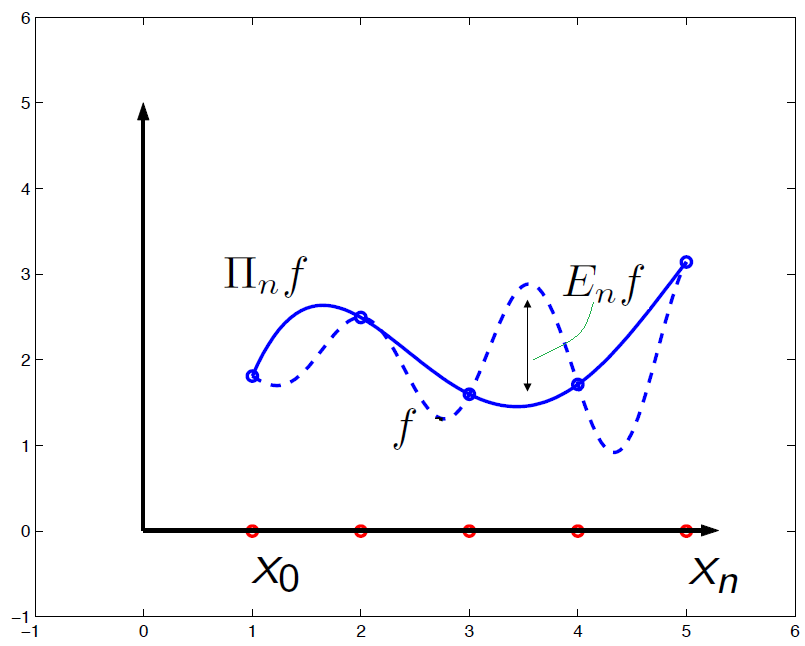
\includegraphics[width=0.4\textwidth]{img/interpolazione-lagrangiana-1.png}
\end{figure}

\noindent
Nel caso di nodi equispaziati, vale la seguente \definition{stima dell'errore massimo dell'interpolatore Lagrangiano}:
\begin{equation}\label{eq: stima dell'errore massimo dell'interpolare Lagrangiano}
	\underset{x \in I}{\max} \left|E_{n} f\left(x\right)\right| \le \dfrac{\left|\underset{x \in I}{\max} f^{\left(n+1\right)\left(x\right)}\right|}{4\left(n+1\right)} \cdot h^{n+1}
\end{equation}

\begin{figure}[!htp]
	\centering
	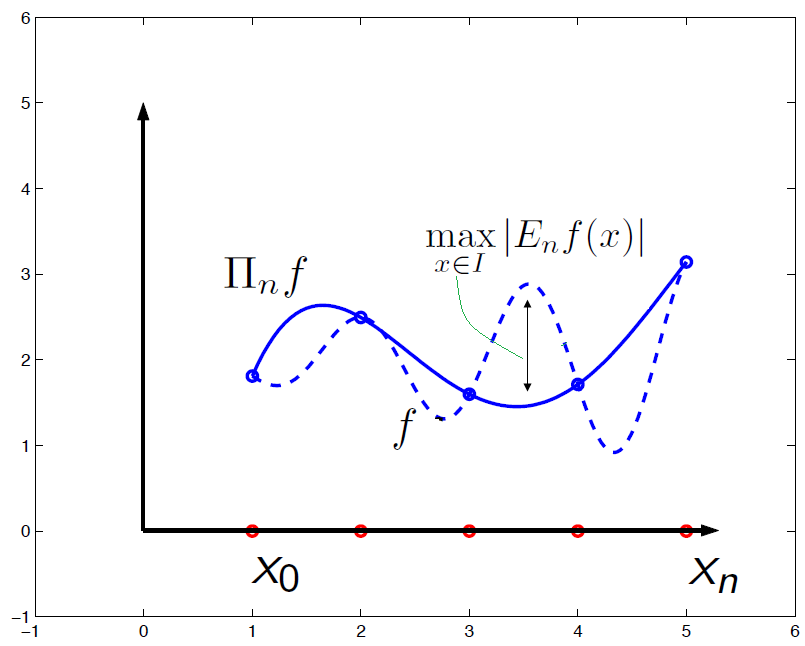
\includegraphics[width=0.4\textwidth]{img/interpolazione-lagrangiana-2.png}
	\label{fig: stima dell'errore massimo dell'interpolatore Lagrangiano}
\end{figure}

\newpage

\subsubsection{Convergenza dell'interpolatore Lagrangiano}

All'aumento delle informazioni a disposizione ($n+1$), idealmente si vorrebbe un \textbf{miglioramento dell'accuratezza di una funzione approssimante}. In particolare, si vorrebbe il seguente risultato:
\begin{equation*}
	\lim\limits_{n \rightarrow \infty} \underset{x \in I}{\max} \left|E_{n}f\left(x\right)\right| = 0
\end{equation*}

\highspace
Dall'equazione \ref{eq: stima dell'errore massimo dell'interpolare Lagrangiano}, a pagina \pageref{eq: stima dell'errore massimo dell'interpolare Lagrangiano}, si può notare che il denominatore della frazione e il termine $h^{n+1}$ tendono a zero quando $n$ tende a infinito. Al contrario, il numeratore non è certo se sia limitato per $n$ che tende a infinito.

\highspace
Difatti, possono esistere casi in cui si ha:
\begin{equation*}
	\lim\limits_{n \rightarrow \infty} \left|\underset{x \in I}{\max} f^{\left(n+1\right)}\left(x\right)\right| = \infty
\end{equation*}
Che portano a:
\begin{equation*}
	\lim\limits_{n \rightarrow \infty} \underset{x \in I}{\max} \left|E_{n} f\left(x\right)\right| = \infty
\end{equation*}
Ovvero alla \textbf{\underline{non} convergenza dell'interpolatore Lagrangiano}.

\begin{examplebox}[: fenomeno di Runge]
	Il \definition{fenomeno di Runge} è un evento che si scatena quando \textbf{l'interpolatore Lagrangiano non raggiunge la convergenza}.
	
	In particolare, in presenza di questo fenomeno, la funzione errore $E_{n}$ presenta delle oscillazioni ai nodi estremi che crescono con il crescere di $n$.
	
	Un esempio di interpolatore $\prod_{12} f$ (in linea continua) calcolato su 13 nodi equispaziati nel caso della funzione di Runge (in linea tratteggiata):
	\begin{equation*}
		f\left(x\right) = \dfrac{1}{\left(1+x^{2}\right)}
	\end{equation*}
	\begin{center}
		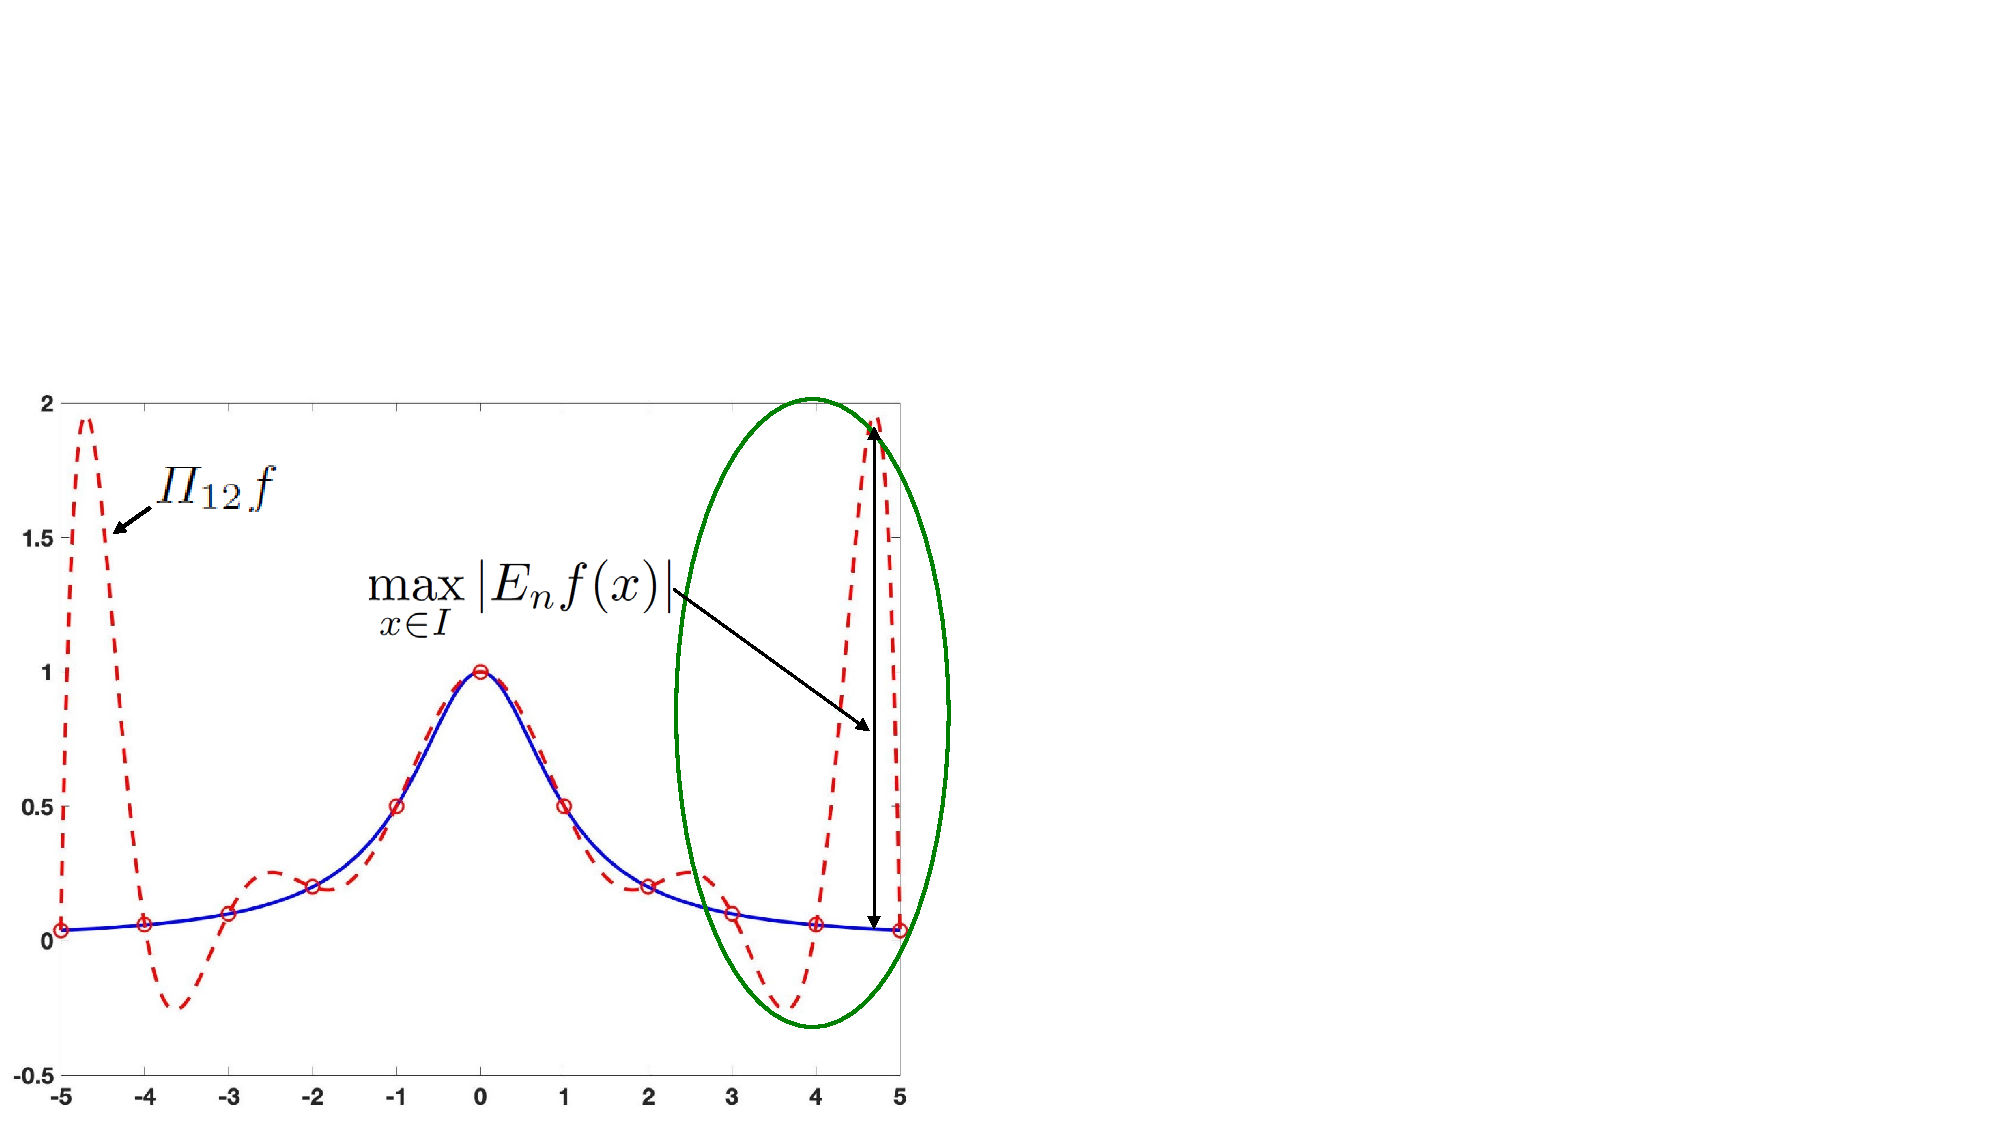
\includegraphics[width=.7\textwidth]{img/fenomeno-di-runge-1.pdf}
	\end{center}
\end{examplebox}